\documentclass[a4paper,12pt, oneside]{book}
\usepackage[utf8]{inputenc}
\usepackage{graphicx}
\usepackage{lmodern}
\usepackage{microtype}
\usepackage{url}
\usepackage{comment}
\usepackage{natbib}
\usepackage{graphicx}
\usepackage{caption}
\captionsetup[table]{skip=10pt}
%Borde de la figuras
\usepackage{framed}
\usepackage[spanish]{babel}
\setcounter{tocdepth}{0}
\setlength{\parskip}{\baselineskip}

\usepackage{multirow}

\usepackage{amsmath}
\usepackage{booktabs}
\usepackage{multicol}
\usepackage{color}
\usepackage{ulem}
\usepackage{pifont}
\usepackage[dvipsnames, svgnames]{xcolor}
\usepackage{tikz}
\usepackage{xcolor}
\usetikzlibrary{calc}
\usepackage{anyfontsize}
\usepackage{sectsty}
\usepackage{kpfonts}
\usepackage[explicit]{titlesec}
\newcommand*\chapterlabel{}
\usepackage{array}
\usepackage{fancyhdr}
\usepackage{nonumonpart}
\pagestyle{plain}
\definecolor{azulUnam}{rgb}{0, 0.24, 0.47}
\definecolor{oroUnam}{rgb}{0.835, 0.624, 0.0588}

\titleformat{\chapter}
{\gdef\chapterlabel{}
	\normalfont\sffamily\Huge\bfseries\scshape}
{\gdef\chapterlabel{\thechapter\ }}{0pt}
{\begin{tikzpicture}[remember picture,overlay]
	\node[yshift=-3cm] at (current page.north west)
	{\begin{tikzpicture}[remember picture, overlay]
		\draw[fill=oroUnam] (0,0) rectangle
		(\paperwidth,3cm);
		\node[anchor=east,xshift=.9\paperwidth,rectangle,
		rounded corners=20pt,inner sep=11pt,
		fill=MidnightBlue]
		{\color{white}\chapterlabel#1};
		\end{tikzpicture}
	};
\end{tikzpicture}
}
\titlespacing*{\chapter}{0pt}{50pt}{-60pt}
\titlespacing*{\section}{0pt}{*2}{*1}


\begin{document}

%\pagestyle{empty}
\thispagestyle{empty}
\begin{tikzpicture}[overlay,remember picture]

% Background color
\fill[
black!2]
(current page.south west) rectangle (current page.north east);

% Rectangles
\shade[
left color=azulUnam, 
right color=azulUnam!60,
transform canvas ={rotate around ={45:($(current page.north west)+(0,-6)$)}}] 
($(current page.north west)+(0,-6)$) rectangle ++(9,1.5);

\shade[
left color=azulUnam,
right color=azulUnam!50,
rounded corners=0.75cm,
transform canvas ={rotate around ={45:($(current page.north west)+(.5,-10)$)}}]
($(current page.north west)+(0.5,-10)$) rectangle ++(15,1.5);

\shade[
left color=oroUnam,
right color=oroUnam!85,
rounded corners=0.3cm,
transform canvas ={rotate around ={45:($(current page.north west)+(.5,-10)$)}}] ($(current page.north west)+(1.5,-9.55)$) rectangle ++(7,.6);

\shade[
left color=oroUnam!80,
right color=oroUnam!60,
rounded corners=0.4cm,
transform canvas ={rotate around ={45:($(current page.north)+(-1.5,-3)$)}}]
($(current page.north)+(-1.5,-3)$) rectangle ++(9,0.8);

\shade[
left color=azulUnam!80,
right color=azulUnam!80,
rounded corners=0.9cm,
transform canvas ={rotate around ={45:($(current page.north)+(-3,-8)$)}}] ($(current page.north)+(-3,-8)$) rectangle ++(15,1.8);

\shade[
left color=oroUnam,
right color=oroUnam!85,
rounded corners=0.9cm,
transform canvas ={rotate around ={45:($(current page.north west)+(4,-15.5)$)}}]
($(current page.north west)+(4,-15.5)$) rectangle ++(30,1.8);

\shade[
left color=azulUnam,
right color=azulUnam!80,
rounded corners=0.75cm,
transform canvas ={rotate around ={45:($(current page.north west)+(13,-10)$)}}]
($(current page.north west)+(13,-10)$) rectangle ++(15,1.5);

\shade[
left color=oroUnam,
rounded corners=0.3cm,
transform canvas ={rotate around ={45:($(current page.north west)+(18,-8)$)}}]
($(current page.north west)+(18,-8)$) rectangle ++(15,0.6);

\shade[
left color=oroUnam,
rounded corners=0.4cm,
transform canvas ={rotate around ={45:($(current page.north west)+(19,-5.65)$)}}]
($(current page.north west)+(19,-5.65)$) rectangle ++(15,0.8);

\shade[
left color=azulUnam,
right color=azulUnam!80,
rounded corners=0.6cm,
transform canvas ={rotate around ={45:($(current page.north west)+(20,-9)$)}}] 
($(current page.north west)+(20,-9)$) rectangle ++(14,1.2);

% Year
\draw[ultra thick,gray]
($(current page.center)+(5,2)$) -- ++(0,-3cm) 
node[
midway,
left=0.25cm,
text width=5cm,
align=right,
black!75
]
{
	{\fontsize{25}{30} \selectfont \bf Pr\'acticas \\ de \\[10pt] Laboratorio}
} 
node[
midway,
right=0.25cm,
text width=4cm,
align=left,
oroUnam]
{
	{\fontsize{60}{86.4} \selectfont 2022}
};

% Title
\node[align=center] at ($(current page.center)+(0,-5)$) 
{
	{\fontsize{60}{72} \selectfont {{Ecofisiolog\'ia}}} \\[1cm]
	{\fontsize{16}{19.2} \selectfont \textcolor{black}{ \bf Alvaro Barreto}}\\[3pt]
	{\fontsize{16}{19.2} \selectfont \textcolor{black}{ \bf Diana Aguilera}}\\[3pt]
	{\fontsize{16}{19.2} \selectfont \textcolor{black}{ \bf Gabriela Gaxiola}}\\[15pt]
	};

\node[inner sep=0pt] (whitehead) at (7,-20)
{\includegraphics[width=.45\textwidth]{ENES.png}};

\end{tikzpicture}


\frontmatter
%\maketitle

\tableofcontents

\mainmatter
\part{Ecofisiol\'ogia de Plantas}

\chapter[Determinaci\'on del potencial h\'idrico]{Potencial h\'idrico}

\begin{huge}
	\begin{center}
		\textbf{Determinaci\'on del potencial h\'idrico en tejido con el m\'etodo gravim\'etrico}
	\end{center}
\end{huge}

\hspace{0.2cm}

\section{Introducci\'on}

% El agua en la planta
% Faltan citas 
El agua presenta un rol importante en la vida de la planta. Adem\'as, es considerada un nutriente porque es la forma en que las plantas absorben y asimilan los \'atomos de hidr\'ogeno durante la fotos\'intesis. Por otra parte, una de sus principales funciones es la de transporte, distribuci\'on de nutrientes, y metabolitos en la planta \citep{kirkham2014principles}. 

La principal magnitud que rige los movimientos del agua es el potencial qu\'imico ($\mu$), esto es la variaci\'on de energ\'ia libre ($\Delta G$) del agua en un punto a causa de los cambios en el volumen molar del agua. El potencial h\'idrico ($\Psi$) se deriva de el potencial qu\'imico, en otras palabras, $\Psi$ es la cantidad de trabajo que hay que proporcionar a una unidad de masa de agua vinculada a los tejidos de una planta, para transformarla a un estado de referencia como es el agua pura (con similar  presi\'on atmosf\'erica y temperatura) con su valor fijado en cero \citep{roger2001handbook}.

La conexi\'on entre $\mu$ y $\Psi$ es:

$$\Psi = \frac{\mu_w - \mu_w^{*}}{V} $$ 

Donde:

\begin{itemize}
	\item $\Psi = $ es el potencial h\'idrico y es expresado en unidades de presi\'on como pascal;
	\item  $\mu_w = $ el potencial qu\'imico del agua en el sistema bajo consideraci\'on;
	\item $\mu_w^{*} = $ potencial qu\'imico del agua pura a presi\'on atmosf\'erica y a la misma temperatura que el sistema en consideraci\'on;
	\item $V = $ volumen molar del agua (18 cm$^3$/mol), es decir, el volumen de un mol de agua.
\end{itemize}

Desde, $\Psi$ es una expresi\'on de estado de $\Delta G$ del agua, este es afectado por todos los factores en el cual cambian la $\Delta G$ o actividad qu\'imica de las mol\'eculas de agua. 

En consecuencia $\Psi$ es incrementado por: (1) desarrollo de presi\'on hidrost\'atica (turgencia); y (2) incremento de temperatura. $\Psi$ es disminuido por: (1) adici\'on de s\'olidos; (2) fuerzas m\'atricas que adsorben agua; (3) presi\'on negativa; y (4) reducci\'on de temperatura.

\subsection{Componentes del potencial h\'idrico}

El t\'ermino potencial h\'idrico fue propuesto por \citet{slatyer1960terminology}, en sus estudios de las relaciones planta-suelo-agua. 

En un sistema particular, el potencial h\'idrico puede ser expresado como la suma de cuatro componentes:

$$\Psi = \Psi_p + \Psi_s + \Psi_m + \Psi_g$$

Donde:

\begin{itemize}
	\item  $\Psi_p = $ potencial de presi\'on. Es el resultado de la presi\'on hidrost\'atica en la c\'elula, que ocurre cuando la presi\'on celular equilibra la diferencia de potencial hídrico entre el ambiente que rodea a la célula y el citoplasma;
	
	\item $\Psi_s = $ potencial osm\'otico. Es consecuencia a la presi\'on de solutos disueltos, disminuye la energ\'ia del agua y siempre es negativo;
	
	\item $\Psi_m = $ potencial m\'atrico. Es producto de fuerzas en las superficies de los s\'olidos. Su principal contribuci\'on es la fuerzas que retienen las mol\'eculas de agua por capilaridad, adsorci\'on e hidrataci\'on, en la superficie de las paredes celulares y el citoplasma;
	
	\item $\Psi_g = $ componente gravitacional. Es producto de la diferencia en energ\'ia potencial como resultado de la diferencia en altura con el nivel de referencia. Por lo general aumenta 0.01 MPa/m por encima del nivel del suelo. 
\end{itemize}

El potencial m\'atrico en las c\'elulas por lo general su efecto es muy peque\~no que puede ser ignorado, sin embargo, es particularmente importante en las primeras etapas de la absorción de agua por parte de las semillas secas (llamada imbibici\'on) y cuando se considera el agua retenida en los suelos \citep{hopkins2009introduction}. El componente gravitacional suele ser considerado cuando se mide el movimiento en los \'arboles. Por lo tanto, el potencial h\'idrico puede ser definido como: 

$$\Psi = \Psi_p + \Psi_s$$

En relaci\'on a la idea anterior, podemos replantear la fuerza motriz del movimiento de agua como el \textbf{gradiente del potencial h\'idrico} (Fig.~\ref{fig:gradiente}), en otras palabras, el agua se desplazar\'a de una regi\'on de $\Psi$ menos negativo hacia una regi\'on de $\Psi$ m\'as negativa. 

\begin{figure}[h]
	\begin{leftbar}
	
	\includegraphics[width=\textwidth]{Gradiente_potencial}
	\centering
	\caption{\textit{Diagrama en el que se ilustran las contribuciones del potencial osmótico ($\Psi_s$), el potencial de presión ($\Psi_p$ ) y el potencial hídrico ($\Psi$) al movimiento del agua entre las células (Adaptado de \citealt{hopkins2009introduction}). Los valores de $\Psi$ se expresan en MPa.}}
	\label{fig:gradiente}
	
	\end{leftbar}
	
\end{figure}

La forma de calcular $\Psi_s$ para muchas soluciones biol\'ogicas es con la relaci\'on de van't Hoff:

$$ \Psi_s = -C i R T$$

Donde:

\begin{itemize}
	\item $C = $ concentraci\'on de soluto expresada en moles
	\item $i = $ constante de ionizaci\'on, para la sacarosa es igual a 1
	\item $R = $ constante de gases, su valor es 0.00831 Kg MPa/mol/K
	\item $T = $ Temperatura en grados Kelvin ($^\circ$C + 273) 
\end{itemize}

\subsection{Medici\'on del potencial h\'idrico}

El potencial h\'idrico para diferentes tejidos en plantas puede ser medido por los siguientes m\'etodos:

\begin{enumerate}
	\item Psicrom\'etrico de termopares
	\item M\'etodo de c\'amara de presi\'on
	\item M\'etodo gravim\'etrico 
	\item M\'etodo sonda de presi\'on
\end{enumerate}


\subsection{Principio}

Las c\'elulas vegetales ajustan constantemente su estado h\'idrico a consecuencia de los cambios en el contenido de agua del entorno y a variaciones del estado metab\'olico. Cuando una c\'elula se encuentra en un entorno isot\'onico, se puede decir que la c\'elula se encuentra en \textbf{plasm\'olisis incipiente} (Fig. ~\ref{fig:pasmolisis}) que dicha condici\'on el protoplasto apenas llena el volumen celular. En consecuencia, cuando una c\'elula se encuentra en dicho estado el $\Psi_p$ equivale a cero y el $\Psi$ de la c\'elula es igual al $\Psi_s$ \citep{NOBEL2020491}. Cabe considerar, por otra parte que si la c\'elula se encuentra en un soluci\'on hipot\'onica (agua destilada), es decir, una soluci\'on con menor contenido de solutos, debido a esto el agua entrar\'a a la c\'elula y provocar\'a un diluci\'on en el contenido vacuolar generando un mayor potencial de presi\'on. El agua dejar\'a de entrar a la c\'elula cuando el $\Psi_s$ y $\Psi_p$ se equilibren, en consecuencia el potencial h\'idrico equivale a cero ($\Psi = 0$). Por otra parte, cuando la c\'elula est\'a sumergida en una soluci\'on hipert\'onica, es decir, una soluci\'on con mayor cantidad de solutos; el gradiente del $\Psi$ favorece la p\'erdida de agua en la c\'elula. Dicha condici\'on se le conoce como plasm\'olisis generando que el protoplasto se separe de la pared celular. 

\begin{figure}[h]
	
	\begin{leftbar}
		
		\includegraphics[width=\textwidth]{Plasmolisis}
		\centering
		\caption{\textit{Estado de la c\'elula cuando se encuentra en diferentes condiciones del medio extracelular.}}
		\label{fig:pasmolisis}
		
	\end{leftbar}

\end{figure}

De este modo cuando un tejido se sumerge en soluciones con potencial osm\'otico conocido estos cambiaran su peso, ya que el volumen celular cambia dependiendo de la concentraci\'on osm\'otica de la soluci\'on. Por lo tanto, en est\'a pr\'actica vamos a conocer el potencial osm\'otico de la papa \textit{Solanum tuberosum} para estimar el punto isosmotico.


\section{Objetivo general}

Determinar el potencial h\'idrico en papa \textit{Solanum tuberosum}.

\section{Objetivo espec\'ifico}

\begin{enumerate}
	
	\item Determinar el peso de los tejidos en papa \textit{Solanum tuberosum} con diferentes soluciones de sacarosa. 
	
	\item Evaluaci\'on del potencial h\'idrico en tejidos de papa \textit{Solanum tuberosum}.
	
\end{enumerate}

\section{Materiales}

\subsection{Material requerido}

\begin{enumerate}
	\item 10 tubos c\'onicos
	\item Nueve vasos de precipitados 
	\item Piceta de agua destilada
	\item Probeta de 100 mL
	\item Cinta adhesiva
	\item Agua destilada
	\item Sacarosa (masa molecular 342.3 g/mol)
	\item Azul de metileno
	\item Papa
	%\item Tub\'erculo de cebolla
\end{enumerate}

\subsection{Material por grupo}

\begin{enumerate}
	\item Balanza anal\'itica
	\item Papel secante
	\item Azul de metileno
\end{enumerate}

\section{Metodolog\'ia}

\subsection{Preparaci\'on de reactivos}

Necesitamos calcular la cantidad de sacarosa para preparar 100 mL de soluci\'on en las siguientes concentraciones molares \footnote{\footnotesize Una soluci\'on 1 molar (1 M) contiene el peso molecular de una sustancia (en gramos) por 1L de soluci\'on.} : \textbf{0.05, 0.1, 0.2, 0.25, 0.3, 0.4, 0.5, 0.7, 0.8 M}.

El peso molecular de la sacarosa es de 342.3 g/M. Por lo tanto, primero calculamos cu\'antos gramos se necesitan para obtener 1 L de soluci\'on a 0.05 M. 

\newpage

Lo resolvemos por una simple regla de tres:

$$\frac{342.3 \text{ g}}{1 \text{ M}} = \frac{\text{\textbf{\textit{x}}} \text{ g}}{0.05 \text{ M}}$$

Se obtiene:

$$ \text{\textbf{\textit{x}}} \text{ g} = \frac{342.3 \text{ g}}{1 \text{ M}} \times 0.05 \text{ M} = 17.12 \text{ g} $$

Por tanto, para preparar 1L de sacarosa a 0.05M, se requiere 17.12g sacarosa.

Establecemos una segunda regla de tres para calcular la cantidad de sacarosa necesaria para preparar 100 mL de un soluci\'on 0.05 M. 

$$\frac{17.12 \text{ g}}{1000 \text{ mL}} = \frac{\text{\textbf{\textit{x}}} \text{ g}}{100 \text{ mL}}$$

Resolviendo la expresi\'on:

$$ \text{\textbf{\textit{x}}} \text{ g} = \frac{17.12 \text{ g}}{1000 \text{ mL}} \times 100 \text{ mL} = 1.71 \text{ g} $$

Por lo tanto, para preparar 100 mL de una soluci\'on de sacarosa a 0.05 M, se necesita disolver 1.17 g de sacarosa en un volumen final de 100 mL de agua destilada.

Para las siguientes concentraciones los pesos estimados son:

\begin{tabular}{p{0.33\textwidth}p{0.33\textwidth}p{0.33\textwidth}}
 0.05 M = 1.71 g  &  0.25 M = 8.56 g & 0.5 M = 17.12 g \\
0.1 M = 3.42 g & 0.3 M = 10.27 g & 0.7 M = 23.96 g \\
 0.2 M = 6.85 g & 0.4 M = 13.69 g & 0.8 M = 27.38 g
\end{tabular}

\subsection{Procedimiento}

\begin{itemize}
	\item Tomar 10 secciones homog\'eneas de un tub\'erculo de papa (Ver la figura~\ref{fig:Diagrama_1}).
	\item Pesar cada secci\'on en la balanza anal\'itica (peso inicial).
	\item Introduzca una secci\'on por cada concentraci\'on de sacarosa y agregar una gota de azul de metileno. Dejar incubar por 45 minutos.
	\item Despu\'es del tiempo de incubaci\'on, remover las secciones y secar el exceso de soluci\'on con papel absorbente.
	\item Pesar las secciones de papa en el orden que fueron colocadas.
	\item Anotar los datos en el cuadro~\ref{resultados:potencial} y calcular el porcentaje de cambio en peso de cada muestra. 
\end{itemize}

\begin{figure}[h]
	
	\begin{leftbar}
	
	\includegraphics[width=\textwidth]{diagrama.png}
	\centering
	\caption{\textit{Diagrama de procedimientos para el m\'etodo volumen/peso para la determinaci\'on del potencial h\'idrico en tejido de papa.}}
	\label{fig:Diagrama_1}
	
	\end{leftbar}
	
\end{figure}

\section{Resultados}

\begin{table}[h!]
	\caption{Datos de cambio de peso en porciones de papa incubadas en diferentes soluciones de sacarosa.}
	
	\label{resultados:potencial}
	\centering
	\begin{tabular}{|p{0.17\textwidth}|p{0.17\textwidth}|p{0.17\textwidth}|p{0.17\textwidth}|p{0.17\textwidth}|}
	
	\hline  &&&& \\
	Soluci\'on sacarosa (M) & Peso inicial (g) & Peso final (g) & $\Delta$ peso$^\dagger$ (g) & Porcentaje $\Delta$ peso$^\mp$ \\
	&&&& \\
	\hline 
	0.00 &&&& \\
	0.05 &&&& \\
	0.10 &&&& \\
	0.20 &&&& \\
	0.25 &&&& \\
	0.30 &&&& \\
	0.40 &&&& \\
	0.50 &&&& \\
	0.70 &&&& \\
	0.80 &&&& \\

	\hline 

	\multicolumn{5}{l}{\footnotesize $^\dagger$ $\Delta$ peso = Peso final - Peso inicial. } \\
	\multicolumn{5}{l}{\footnotesize $^\mp$ Porcentaje $\Delta$ peso = $\Delta$ peso / Peso inicial $\times$ 100 }	
	
	\end{tabular}
\end{table}

\begin{itemize}
	\item Elaborar un gr\'afico (fig.~\ref{fig:ejem_concentracion}) del porcentaje de cambio en peso del tejido en funci\'on de la concentraci\'on de sacarosa (M).
	\item Determinar la concentraci\'on de sacarosa en la cual no se presento un cambio en el peso del tejido.
	\item Calcular el $\Psi_s$ de la soluci\'on con la ecuaci\'on de van't Hoff. 
\end{itemize}

\begin{figure}[h!]
	
	\begin{leftbar}
		
		\includegraphics[width=\textwidth]{graf_cambio}
		\centering
		\caption{\textit{Representaci\'on del cambio en peso en funci\'on de la concentraci\'on de sacarosa.}}
		\label{fig:ejem_concentracion}
		
	\end{leftbar}
	
\end{figure}


\section{Cuestionario}

\begin{enumerate}
	\item \textquestiondown De que forma el concepto de potencial h\'idrico ayuda a explicar los movimientos de agua en los tejidos vegetales?
	\item Cuando una c\'elula est\'a totalmente turgente, \textquestiondown cu\'al de las siguientes opciones equivale a cero?
		\begin{itemize}
			\item Potencial osm\'otico
			\item Potencial h\'idrico
			\item Presi\'on de turgencia
		\end{itemize}
	%\item Utilizando un corte delgado en la epidermis de una cebolla, se obtiene los siguientes datos; presenta un intercambio nulo con una soluci\'on de $ClNa$ 0.150 M a 25 $^\circ$C; la plasm\'olisis incipiente se presenta en una soluci\'on de $ClNa$ 0.293 M a la misma temperatura. Determine los distintos componentes del potencial h\'idrico de las c\'elulas en la epidermis de cebolla en el estado inicial y final del la plam\'olisis. Considerando que $\Psi_m$ es casi nulo y las membranas no son permeables al $ClNa$. 
\end{enumerate}


%\chapter[Efecto de la concentraci\'on osm\'otica y temperatura en la imbibici\'on y germinaci\'on de semillas de papaya]{Germinaci\'on}

\begin{Huge}
	\begin{center}
		\textbf{Determinar la imbibici\'on y germinaci\'on de semillas de papaya en diferentes temperaturas y condiciones osm\'oticas}
	\end{center}
\end{Huge}

\section{Introducci\'on}

La semilla es una estructura que se desarrolla a partir del ovulo despu\'es de la fertilizaci\'on. Est\'a constituido por un embri\'on, el tejido que almacena los nutrientes, y las cubiertas seminales. Las semillas de las angiospermas est\'an contenidas dentro del fruto que se desarrolla de las paredes del ovario, sin embargo, en las plantas gimnospermas la semilla est\'a expuesta y no se encuentra dentro del fruto.

Cabe resaltar que la semillas se encuentran extremadamente deshidratadas, en consecuencia las reacciones metab\'olicas son escasamente detectables. Est\'a caracter\'istica permite al embri\'on sobrevivir en condiciones adversas por largos periodos de tiempo. La semilla, por tanto, est\'a en una fase quiescente\footnote{La definici\'on de la RAE es que est\'a quieto pudiendo tener movimiento propio} y representa una etapa normal en el ciclo de vida de una planta. 

La germinaci\'on es la reanudaci\'on del crecimiento del embri\'on. En condiciones de campo, la tasa de germinaci\'on puede ser controlada por el potencial h\'idrico del suelo y la temperatura. El potencial h\'idrico del suelo es la suma del potencial m\'atrico y el componente de solutos solubles que posee. Con respecto a la temperatura est\'a depende de la especie, por lo tanto, el rango de temperatura determina el h\'abitat y la distribuci\'on geogr\'afica en las plantas.

El proceso de germinaci\'on da inicio cuando la semilla absorbe agua y dicho proceso se le conoce como imbibici\'on. La rehidrataci\'on de los tejidos de la semilla es llevada a cabo por fuerzas matricas que son el resultado de la atracción química y electrostática del agua hacia las paredes celulares y materiales celulares hidrof\'ilicos. En consecuencia, la semilla se hincha causando una ruptura de las cubiertas seminales permitiendo al embri\'on emerger \citep{hopkins2009introduction}. 

\begin{table}[h]
	\caption{Intervalo de Temperaturas optimas, m\'aximas, media, y potencial h\'idrico para la germinaci\'on de semillas de plantas de cultivo.}
	\label{tabla:germinacion}
	\begin{tabular}{p{0.17\textwidth}p{0.17\textwidth}p{0.17\textwidth}p{0.17\textwidth}p{0.17\textwidth}}
		\hline
		Cultivo & T$_{opt}$ & T$_{50\%}$ & T$max$  & $\Psi$ \\ % Topt , Tb50% germ, Tmax 
		\hline
		Trigo &   & 1.2-1.6 & 30 & -2.9 \\
		
		Arroz & 30 & 10 &  &  \\

		Ma\'iz & 32 & 8-8.2  &   & -1.6 \\

		Sorgo & 35.8 & 11 & 45 &  \\
		
		Algod\'on & 33-36 & 14 & 40  & -1 \\
		
		Soya & 34 & 4-10 & 40-50 &  \\
		
		Frijoles & 32 & 6.6 & 48 & -2.3 \\
		\hline
		\multicolumn{5}{l}{\footnotesize Valores obtenidos de \citet{drr2014lrag}}
	\end{tabular}
\end{table}

Con respecto a la temperatura, puede influenciar la tasa de imbibici\'on y en consecuencia el proceso de germinaci\'on. En el cuadro \ref{tabla:germinacion} se presentan las temperaturas optimas para la germinaci\'on, as\'i como los valores m\'aximos. 

\section{Principio}

El agua en diferentes concentraciones osm\'oticas puede causar un estr\'es salino. Por lo tanto, puede afectar los procesos de imbibici\'on y germinaci\'on de la semilla al disminuir el potencial h\'idrico del agua. 

% Fundamentos de fisiolog\'ia pagina 563

% Hopkins Introduction to plant physiology pag 301

% Plant physilogy Sinauer Associates

\section{Objetivo general}

Evaluar el efecto de diferentes concentraciones osm\'oticas en la imbibici\'on y germinabilidad de las semillas de papaya en diferentes temperaturas. 

\section{Obejetivo espec\'ifico}

\begin{enumerate}
	\item Determinar el porcentaje de imbibici\'on de semillas de papaya \textit{Carica papaya} en soluciones de 0.5 y 1.0M de $NaCL$ en temperatura ambiente y baja temperatura (4-5 $^\circ$C).
	\item Determinar el porcentaje de germinaci\'on de semillas de papaya \textit{Carica papaya} en soluciones de 0.5 y 1.0M de $NaCL$ en temperatura ambiente y baja temperatura (4-5 $^\circ$C).
\end{enumerate}

\section{Materiales}

\subsection{Material requerido }

\begin{enumerate}
	\item 18 platos petri o vasos de pl\'astico
	\item Matraz aforado de 1 L
	\item Agua destilada
	\item 100g $NaCL$
	\item Semillas de papaya
\end{enumerate}

\subsection{Material por grupo}

\begin{enumerate}
	\item Balanza anal\'itica
	\item Papel secante
\end{enumerate}

\section{Metodolog\'ia}

\subsection{Preparaci\'on de reactivos}

Para preparar la soluci\'on de 0.5 y 1.0M de $NaCl$ se disuelve 29.25 y 58.5g de $NaCl$ en un litro de agua destilada, respectivamente. 

\subsection{Procedimiento}  

Conseguir semillas en un vivero o centro autorizado. Tambi\'en se puede ocupar las que se encuentran dentro del fruto, si eliges est\'a opci\'on tienes que lavar muy bien la semilla para que no tenga ning\'un residuo org\'anico. Una forma muy sencilla de seleccionar semillas viables es dejarlas en un recipiente con agua por 10 minutos y desechar las semillas que flotan. Luego se procede a desinfectar las semillas, por tanto, debes sumergirlas en agua, agregar cuatro gotas de cloro y esperar cinco minutos. Posteriormente, se enjuagan bien con agua destilada o con agua de garraf\'on unas tres o cuatro veces. 

\begin{figure}[h]
	
	\begin{leftbar}
		
		\includegraphics[width=0.5\textwidth]{Petri2.png}
		\centering
		\caption{\textit{\textbf{A}: colocaci\'on aleatoria de los tratamientos para la determinaci\'on del porcentaje de imbibici\'on y germinaci\'on en soluciones de 0.5, 1.0M de NaCl, y agua destilada como control. \textbf{B}: tratamientos condici\'on de temperatura ambiente y baja temperatura.}}
		\label{fig:petri}
		
	\end{leftbar}
	
\end{figure}

A continuaci\'on se forman nueve grupos de semillas por condici\'on de temperatura, cada grupo puede tener entre tres a cuatro semillas. Se registra el peso inicial de cada semilla. Luego se coloca un grupo de semilla en cada plato petri (o en vaso de pl\'astico desechable) sobre papel absorbente (Figura \ref{fig:petri}). Posteriormente, se agrega el mismo volumen de soluci\'on con una jeringa de 5 mL y se cubre el plato petri. Los tratamientos consisten en un control con agua destilada (o de garraf\'on), soluciones de 0.5 y 1.0M de NaCl, por triplicado cada tratamiento. 

Despu\'es de dos o cuatro d\'ias se vuelve a registrar el peso de las semillas, y el n\'umero de semillas germinadas. Por lo tanto, se calcula el porcentaje de imbibici\'on y germinaci\'on, respectivamente.

$$\text{Imbibici\'on} (\%) = \frac{P_2 - P_1}{P_1} \times 100$$ 

Donde:

\begin{itemize}
	\item $P_1 =$ peso inicial del lote de semillas (en cada plato petri).
	\item $P_2 =$ peso del lote de semillas, despu\'es del tiempo indicado.
\end{itemize}

$$\text{Germinaci\'on} (\%) = \frac{SG}{TS} \times 100$$

Donde:

\begin{itemize}
	\item $SG =$ n\'umero de semillas germinadas.
	\item $TS =$ n\'umero total de semillas. 
\end{itemize}

Tome en cuenta las siguientes precauciones: seleccionar semillas sanas, evitar contaminaci\'on y el tratamiento a temperatura ambiente debe estar en un lugar seco y con sombra. Las muestras deben mantenerse h\'umedas durante el tiempo del experimento, por lo tanto, deben de taparse bien. 

\section{Resultados}

Los resultados obtenidos se pueden presentar en el cuadro \ref{resultados:germinacion}.

\begin{table}[h!]
	\caption{Datos de porcentaje de imbibici\'on y germinaci\'on de semillas de papaya en diferentes concentraciones de $NaCl$ y temperaturas de incubaci\'on.}
	
	\label{resultados:germinacion}
	\centering
	\begin{tabular}{p{0.17\textwidth} p{0.17\textwidth} p{0.17\textwidth} p{0.17\textwidth} p{0.17\textwidth}}
		
		\hline  &&&& \\
		Temperatura & Soluci\'on (M) & Repetici\'on & Imbibici\'on (\%) & Germinaci\'on (\%) \\
		\hline 
		
		\multirow{9}{*}{Ambiente}& \multirow{3}{*}{Control} & A1 & & \\ 
															%\cline{3-5}
														   & & A2 & & \\
														   %\cline{3-5}
														   & & A3 & & \\
														   \cline{2-5}
														   
								 & \multirow{3}{*}{0.5}		 & B1 & & \\
															 &&B2&& \\
															 &&B3&& \\
															\cline{2-5} 
		 &\multirow{3}{*}{1.0}& C1 && \\
		&&C2&& \\
		 &&C3&& \\
		
		\hline 
		\multirow{9}{*}{4-5 $^\circ$C}& \multirow{3}{*}{Control} & A1 & & \\ 
		& & A2 & & \\
		& & A3 & & \\
		\cline{2-5} 
		& \multirow{3}{*}{0.5}		 & B1 & & \\
		&&B2&& \\
		&&B3&& \\
		\cline{2-5} 
		&\multirow{3}{*}{1.0}& C1 && \\
		&&C2&& \\
		&&C3&& \\
		
		\hline 
					
	\end{tabular}
\end{table}



\section{Cuestionario}

\begin{enumerate}
	\item \textquestiondown C\'omo explica la relaci\'on entre la concentraci\'on osm\'otica y el porcentaje de imbibici\'on?
	\item \textquestiondown Por qu\'e influy\'o la temperatura en el porcentaje de germinaci\'on?
	
\end{enumerate}

%\chapter[Extracci\'on de pigmentos vegetales y cromatograf\'ia]{Clorofila}

\begin{Huge}
	\begin{center}
		\textbf{Extracci\'on de pigmentos vegetales y cromatograf\'ia}
	\end{center}
\end{Huge}

\section{Introducci\'on}

Los mayores pigmentos fotosint\'eticos son la clorofilas, carotenoides, y ficobilinas. Entre ellos, las clorofilas y los carotenoides son los pigmentos m\'as abundantes en las hojas de las plantas superiores y otros organismos fotosint\'eticos. Las microalgas son una fuente importante de colorantes naturales, como la ficocianina, ficoeritrina, y astaxantina, que están ganando un mayor interés que los colorantes sintéticos debido a sus características no tóxicas y no cancerígenas. La ficocianina y la ficoeritrina son pigmentos fotosintéticos de color azul y rojo, respectivamente, que se encuentran en microalgas, cianobacterias, rodofitas y criptofitas.

Las clorofilas son los pigmentos que dan a las plantas su color verde caracter\'istico. Constituyen aproximadamente el 4\% del cloroplasto (en peso seco). La clorofila\textit{-b} (Chl\footnote{Chl, de la palabra en inglés "chlorophyll"} a) se presenta como un tercio del contenido de la clorofila\textit{-a}. Por lo tanto, la clorofila\textit{-a} (Chl b) es un componente de los centros de reacción fotosintéticos y podemos considerarla como el pigmento fotosintético esencial. 

La Chl a muestra dos bandas de absorción principales: una en el rojo, con un máximo alrededor de 660 nm y un pico de absorción importante en el extremo azul a violeta del espectro visible (máximo alrededor de 435 nm). La Chl b muestra también dos bandas de absorción importantes: una en el rojo-naranja del espectro visible, con un máximo a 650 nm, y la otra en el rango del azul.

\subsection{Principio}

Los pigmentos fotosint\'eticos son solubles en diferentes solventes org\'anicos. Con base a las diferencias de solubilidad de esos pigmentos en diferentes solventes, ellos pueden ser separados e identificados. 

\section{Objetivo general}

Extraer los pigmentos fotosint\'eticos presentes en las hojas de plantas herbáceas y separarlos por el m\'etodo de cromatograf\'ia.

\section{Objetivos espec\'ificos}

\begin{enumerate}
	\item Extracci\'on de pigmentos fotosint\'eticos de hojas de lechuga y espinaca.
	\item Comparar los pigmentos extra\'idos con cromatograf\'ia de papel.
\end{enumerate}

\section{Materiales}

\subsection{Material requerido}

\begin{enumerate}
	\item Medio litro de alcohol isopropílico 
	\item Dos vasos de vidrio con tapa
	\item Dos morteros con pistilo
	\item Dos lapices
	\item Dos filtros para caf\'e
	\item Dos vasos de precipitado de 500 mL
	\item Una cinta adhesiva
\end{enumerate}

\subsection{Material por grupo}

\begin{enumerate}
	\item Parrilla de calentamiento
	\item Un vaso de precipitado de 1 L
\end{enumerate}

\section{Metodolog\'ia}

\subsection{Preparar reactivos}

Poner a calentar un litro de agua en la parrilla de calentamiento y los filtros para caf\'e recortarlos en tiras de dos cent\'imetros de ancho y el largo debe ser unos tres cent\'imetros mayor que la altura del vaso de vidrio.

\subsection{Procedimiento}

Tomar unas hojas y triturarlas en el mortero hasta dejar una pasta. Luego vamos a colocar dicha pasta en el vaso de vidrio y agregamos alcohol isoprop\'ilico hasta cubrirlo. Cerramos muy bien el vaso y lo colocamos dentro de un vaso de precipitado de 500 mL, posteriormente agregamos agua caliente. Dejarlo por lo menos media hora y si el agua se enfr\'ia podemos reemplazarla para mantener la temperatura del agua caliente.

A continuaci\'on, retiramos el vaso de vidrio y quitamos la tapa. Con la cinta adhesiva pegamos una tira de papel al l\'apiz y lo colocamos sobre el vaso de vidrio(ver figura~\ref{fig:cromatografia}). De est\'a manera la cinta quedar\'a dentro del vaso y la parte inferior de la tira estar\'a sumergida en el alcohol isopropílico entre una o dos horas.

Al terminar le puedes tomar una fotograf\'ia con tu celular o c\'amara fotogr\'afica. Para presentar la diferencia de colores entre las cromatograf\'ias de las hojas de lechuga y espinaca vamos utilizar el sistema RGB. El modo de color RGB ("Red", "Green", y "Blue") es la composici\'on de los colores primarios en funci\'on de su intensidad. Por lo general, la intensidad de cada uno de los componentes se encuentran en una escala de 0 a 255. Por ejemplo, los colores de la UNAM son azul (RGB: 0, 61, 121) y oro (RGB: 213, 159, 15). En algunos casos se puede agregar un cuarto valor que representa la transparencia. 

Para conocer los colores en el sistema RGB deben subir su fotograf\'ia a la pagina web https://imagecolorpicker.com/ y seguir los siguientes pasos:

\begin{enumerate}
	\item Abrir la pagina https://imagecolorpicker.com/ 
	\item Dar clic en \textbf{Use Your Image} para cargar la imagen
	\item Poner el cursor sobre la imagen y dar clic en la parte que necesitamos conocer su color en t\'erminos de RGB
	\item Copiar los primeros tres valores 
\end{enumerate}


\begin{figure}[h]
	
	\begin{leftbar}
		
		\includegraphics[width=0.5\textwidth]{cromatofrafia.png}
		\centering
		\caption{\textit{Procedimiento para extraer los pigmentos fotosint\'eticos presentes en las hojas de las plantas y separarlos por el m\'etodo de cromatograf\'ia.}}
		\label{fig:cromatografia}
		
	\end{leftbar}
	
\end{figure}

\section{Resultados}

Presentar las fotograf\'ias y sus valores respectivos en el sistema RGB

\section{Cuestionario}

\begin{enumerate}
	\item \textquestiondown Por qu\'e la clorofila es verde?
	\item \textquestiondown Por qu\'e la clorofila \textit{-a} es m\'as abundante?
	\item La energ\'ia de la luz irradiada es inversamente proporcional a la longitud de onda. \textquestiondown verdadero o falso?
	\item \textquestiondown Cu\'al es la importancia de la expresi\'on anterior, con respecto al pico de absorción de la  clorofila \textit{-a}?
	\item \textquestiondown Cu\'al planta cree usted que present\'o una mayor cantidad de clorofila en sus hojas?
\end{enumerate}



%\chapter[Pigmentos vegetales como indicadores de pH]{Pigmentos}

\begin{Huge}
	\begin{center}
		\textbf{Pigmentos vegetales como indicadores de pH}
	\end{center}
\end{Huge}

\section{Introducci\'on}

\subsection{Principio}

\section{Objetivo general}

\section{Objetivos espec\'ificos}

\section{Materiales}

\subsection{Material requerido}

\subsection{Material por grupo}

\section{Metodolog\'ia}

\subsection{Preparar reactivos}

\subsection{Procedimiento}

\section{Resultados}

\section{Cuestionario}
%\chapter[S\'intesis de almid\'on por el proceso de la fotos\'intesis]{Almid\'on}

\begin{Huge}
	\begin{center}
		\textbf{S\'intesis de almid\'on por el proceso de la fotos\'intesis.}
	\end{center}
\end{Huge}

\section{Introducci\'on}

En la mayor\'ia de las especies, la sacarosa es la principal forma de carbohidrato que se transporta a trav\'es de la planta por el floema. El almid\'on es una reserva de carbohidratos estables e insolubles que est\'a presente en casi todas las plantas. Tanto el almid\'on como la sacarosa se sintetizan a partir de la triosa fosfato que se genera en el ciclo de Calvin. 

El cloroplasto es el sitio de sintesis de almid\'on en las hojas. El almid\'on se sintetiza a partir de la triosa fosfato de la fructosa-1, 6-bisfosfato. El intermediario glucosa-1-fosfato se convierte en ADP-glucosa a través de la ADP-glucosa pirofosforilasa en una reacción que requiere ATP y genera pirofosfato. Como en muchas reacciones biosintéticas, el pirofosfato
se hidroliza a través de una pirofosfatasa inorgánica específica a dos mol\'eculas de ortofosfato, impulsando así la reacción hacia la síntesis de ADP-glucosa. Finalmente, la fracción de glucosa de la ADP-glucosa se transfiere al extremo no reductor de la glucosa terminal de una cadena de almidón en crecimiento, completando as\'i la secuencia de reacci\'on.

\subsection{Principio}

Las concentraciones relativas de ortofosfato y triosa fosfato son los principales factores que controlan si el carbono fijado fotosintéticamente se reparte como almidón en el cloroplasto o como sacarosa en el citosol. El ortofosfato y la triosa fosfato controlan la actividad de varias enzimas reguladoras en las vías biosintéticas de la sacarosa y el almidón. La enzima del cloroplasto ADP-glucosa pirofosforilasa es la enzima clave que regula la síntesis de almidón a partir de glucosa-1-fosfato. Esta enzima es estimulada por el 3-fosfoglicerato e inhibida por el ortofosfato. En los cloroplastos iluminados que sintetizan activamente el almidón se suele encontrar una alta proporción de concentración de 3-fosfoglicerato respecto al ortofosfato. Condiciones recíprocas prevalecen en la oscurida.

\section{Objetivo general}

Evaluar la presencia de almid\'on en hojas en condici\'on de oscuridad e iluminaci\'on natural. 

\section{Objetivos espec\'ificos}

\begin{enumerate}
	\item Determinar la presencia de granos de almid\'on en hojas en condici\'on de ausencia de luz solar.
	\item Determinar la presencia de granos de almid\'on en plantas con iluminaci\'on natural.
\end{enumerate}

\section{Materiales}

\subsection{Material requerido}

\begin{enumerate}
	\item Dos vasos de precipitado de 500 mL 
	\item Dos cajas petri
	\item Ba\~no Mar\'ia
\end{enumerate}

\subsection{Material por grupo}

\begin{enumerate}
	\item Un litro de alcohol et\'ilico al 96\%
	\item Soluci\'on de lugol al 10\%
	\item Cuatro microscopios estereoscópicos
\end{enumerate}

\section{Metodolog\'ia}

\subsection{Preparaci\'on de material}

Conseguir dos plantas en un vivero. Una planta se mantendr\'a en oscuridad por dos d\'ias, cubriéndola con una caja de cart\'on. La otra planta se mantendr\'a en un lugar iluminado. 

\subsection{Procedimiento}

En los vasos de precipitado se agregar\'an aproximadamente 100 mL de alcohol et\'ilico. Luego ser\'an colocados en un ba\~no Mar\'ia con agua a punto de ebullici\'on. En uno de los vasos de precipitado se van a sumergir tres hojas de la planta que se mantuvo en la oscuridad y en el otro las hojas de la planta que se mantuvo en un lugar iluminado. Posteriormente, se mantendr\'an en ba\~no Mar\'ia  por 20 min o hasta que las hojas se decoloren. 

Se retiran las hojas y se lavan con agua caliente. Luego, se ponen las hojas en cajas Petri y se agrega soluci\'on de lugol hasta cubrir las hojas. 

Observar las hojas en el microscopio estereosc\'opico y contar las manchas blancas que se formaron.

%Preparar un trozo fino de tubérculo de patata con la ayuda de una cuchilla o navaja. Móntelo sobre un tobogán en una gota de agua. Añadir una gota de solución de yodo (IKI) y cubrir con una tapa de vidrio. Examinar bajo el microscopio de luz. Los granos de almidón se tiñen de azul. Los granos de almidón viejos se tiñen de negro azulado, mientras que el almidón fresco da un color rojo o púrpura.

\section{Resultados}

Tomar fotograf\'ias a las hojas y presentar el conteo de n\'umero manchas por hoja que obtuvieron las plantas que se mantuvieron en un lugar iluminado versus ausencia de luz.

\section{Cuestionario}

\begin{enumerate}
	\item Explique la relaci\'on entre el n\'umero de manchas por hoja en condiciones de oscuridad.
	%\item \textquestiondown Cu\'al es la funci\'on del almid\'on?

\end{enumerate}


%\chapter[Transporte de agua y transpiraci\'on de plantas hal\'ofila]{Transpiraci\'on}

\begin{Huge}
	\begin{center}
		\textbf{Transporte de agua y transpiraci\'on de plantas hal\'ofila}
	\end{center}
\end{Huge}

\section{Introducci\'on}

\subsection{Principio}

\section{Objetivo general}

\section{Objetivos espec\'ificos}

\section{Materiales}

\subsection{Material requerido}

\subsection{Material por grupo}

\section{Metodolog\'ia}

\subsection{Preparar reactivos}

\subsection{Procedimiento}

\section{Resultados}

\section{Cuestionario}

%\part{Ecofisiol\'ogia de organismos acu\'aticos}


\backmatter
% bibliography, glossary and index would go here.
\bibliography{referencias}
\bibliographystyle{apalike}

\end{document}